\documentclass[journal,12pt,onecolumn]{IEEEtran}
%

\usepackage{graphicx}
%\usepackage{amssymb}
%\usepackage{relsize}
\usepackage[cmex10]{amsmath}
%\usepackage{amsthm}
\interdisplaylinepenalty=2500
%\savesymbol{iint}
%\usepackage{txfonts}
%\restoresymbol{TXF}{iint}
%\usepackage{wasysym}
\usepackage{amsthm}
\usepackage{mathrsfs}
\usepackage{txfonts}
\usepackage{stfloats}
\usepackage{cite}
\usepackage{cases}
\usepackage{subfig}
%\usepackage{xtab}
\usepackage{longtable}
\usepackage{multirow}
%\usepackage{algorithm}
%\usepackage{algpseudocode}
\usepackage{enumitem}
\usepackage{mathtools}
%\usepackage{stmaryrd}


%\usepackage{wasysym}
%\newcounter{MYtempeqncnt}
\DeclareMathOperator*{\Res}{Res}
\renewcommand{\baselinestretch}{2}
\renewcommand\thesection{\arabic{section}}
\renewcommand\thesubsection{\thesection.\arabic{subsection}}
\renewcommand\thesubsubsection{\thesubsection.\arabic{subsubsection}}

\renewcommand\thesectiondis{\arabic{section}}
\renewcommand\thesubsectiondis{\thesectiondis.\arabic{subsection}}
\renewcommand\thesubsubsectiondis{\thesubsectiondis.\arabic{subsubsection}}

% correct bad hyphenation here
\hyphenation{op-tical net-works semi-conduc-tor}


\begin{document}
%


\newtheorem{theorem}{Theorem}[section]
\newtheorem{problem}{Problem}
\newtheorem{proposition}{Proposition}[section]
\newtheorem{lemma}{Lemma}[section]
\newtheorem{corollary}[theorem]{Corollary}
\newtheorem{example}{Example}[section]
\newtheorem{definition}{Definition}[section]
%\newtheorem{algorithm}{Algorithm}[section]
%\newtheorem{cor}{Corollary}
\newcommand{\BEQA}{\begin{eqnarray}}
\newcommand{\EEQA}{\end{eqnarray}}
\newcommand{\define}{\stackrel{\triangle}{=}}

\bibliographystyle{IEEEtran}
%\bibliographystyle{ieeetr}



\providecommand{\nCr}[2]{\,^{#1}C_{#2}} % nCr
\providecommand{\nPr}[2]{\,^{#1}P_{#2}} % nPr
\providecommand{\pr}[1]{\ensuremath{\Pr\left(#1\right)}}
\providecommand{\qfunc}[1]{\ensuremath{Q\left(#1\right)}}
\providecommand{\sbrak}[1]{\ensuremath{{}\left[#1\right]}}
\providecommand{\lsbrak}[1]{\ensuremath{{}\left[#1\right.}}
\providecommand{\rsbrak}[1]{\ensuremath{{}\left.#1\right]}}
\providecommand{\brak}[1]{\ensuremath{\left(#1\right)}}
\providecommand{\lbrak}[1]{\ensuremath{\left(#1\right.}}
\providecommand{\rbrak}[1]{\ensuremath{\left.#1\right)}}
\providecommand{\cbrak}[1]{\ensuremath{\left\{#1\right\}}}
\providecommand{\lcbrak}[1]{\ensuremath{\left\{#1\right.}}
\providecommand{\rcbrak}[1]{\ensuremath{\left.#1\right\}}}
\theoremstyle{remark}
\newtheorem{rem}{Remark}
\newcommand{\sgn}{\mathop{\mathrm{sgn}}}
\providecommand{\abs}[1]{\left\vert#1\right\vert}
\providecommand{\res}[1]{\Res\displaylimits_{#1}} 
\providecommand{\norm}[1]{\lVert#1\rVert}
\providecommand{\mtx}[1]{\mathbf{#1}}
\providecommand{\mean}[1]{E\left[ #1 \right]}
\providecommand{\fourier}{\overset{\mathcal{F}}{ \rightleftharpoons}}
%\providecommand{\hilbert}{\overset{\mathcal{H}}{ \rightleftharpoons}}
\providecommand{\system}{\overset{\mathcal{H}}{ \longleftrightarrow}}
\providecommand{\gauss}[2]{\mathcal{N}\ensuremath{\left(#1,#2\right)}}
	%\newcommand{\solution}[2]{\textbf{Solution:}{#1}}
\newcommand{\solution}{\noindent \textbf{Solution: }}
\providecommand{\dec}[2]{\ensuremath{\overset{#1}{\underset{#2}{\gtrless}}}}
%\numberwithin{equation}{section}
%\numberwithin{problem}{section}

\def\putbox#1#2#3{\makebox[0in][l]{\makebox[#1][l]{}\raisebox{\baselineskip}[0in][0in]{\raisebox{#2}[0in][0in]{#3}}}}
     \def\rightbox#1{\makebox[0in][r]{#1}}
     \def\centbox#1{\makebox[0in]{#1}}
     \def\topbox#1{\raisebox{-\baselineskip}[0in][0in]{#1}}
     \def\midbox#1{\raisebox{-0.5\baselineskip}[0in][0in]{#1}}


% paper title
% can use linebreaks \\ within to get better formatting as desired
\title{Octave for Mathematics}
%
%
% author names and IEEE memberships
% note positions of commas and nonbreaking spaces ( ~ ) LaTeX will not break
% a structure at a ~ so this keeps an author's name from being broken across
% two lines.
% use \thanks{} to gain access to the first footnote area
% a separate \thanks must be used for each paragraph as LaTeX2e's \thanks
% was not built to handle multiple paragraphs
%

%\author{Y Aditya, A Rathnakar and G V V Sharma$^{*}$% <-this % stops a space
\author{G V V Sharma$^{*}$% <-this % stops a space
\thanks{*The author is with the Department
of Electrical Engineering, Indian Institute of Technology, Hyderabad
502205 India e-mail:  gadepall@iith.ac.in.}% <-this % stops a space
%\thanks{J. Doe and J. Doe are with Anonymous University.}% <-this % stops a space
%\thanks{Manuscript received April 19, 2005; revised January 11, 2007.}}
}
% note the % following the last \IEEEmembership and also \thanks - 
% these prevent an unwanted space from occurring between the last author name
% and the end of the author line. i.e., if you had this:
% 
% \author{....lastname \thanks{...} \thanks{...} }
%                     ^------------^------------^----Do not want these spaces!
%
% a space would be appended to the last name and could cause every name on that
% line to be shifted left slightly. This is one of those "LaTeX things". For
% instance, "\textbf{A} \textbf{B}" will typeset as "A B" not "AB". To get
% "AB" then you have to do: "\textbf{A}\textbf{B}"
% \thanks is no different in this regard, so shield the last } of each \thanks
% that ends a line with a % and do not let a space in before the next \thanks.
% Spaces after \IEEEmembership other than the last one are OK (and needed) as
% you are supposed to have spaces between the names. For what it is worth,
% this is a minor point as most people would not even notice if the said evil
% space somehow managed to creep in.



% The paper headers
%\markboth{Journal of \LaTeX\ Class Files,~Vol.~6, No.~1, January~2007}%
%{Shell \MakeLowercase{\textit{et al.}}: Bare Demo of IEEEtran.cls for Journals}
% The only time the second header will appear is for the odd numbered pages
% after the title page when using the twoside option.
% 
% *** Note that you probably will NOT want to include the author's ***
% *** name in the headers of peer review papers.                   ***
% You can use \ifCLASSOPTIONpeerreview for conditional compilation here if
% you desire.




% If you want to put a publisher's ID mark on the page you can do it like
% this:
%\IEEEpubid{0000--0000/00\$00.00~\copyright~2007 IEEE}
% Remember, if you use this you must call \IEEEpubidadjcol in the second
% column for its text to clear the IEEEpubid mark.



% make the title area
\maketitle

%\tableofcontents

%\begin{abstract}
%%\boldmath
%In this letter, an algorithm for evaluating the exact analytical bit error rate  (BER)  for the piecewise linear (PL) combiner for  multiple relays is presented. Previous results were available only for upto three relays. The algorithm is unique in the sense that  the actual mathematical expressions, that are prohibitively large, need not be explicitly obtained. The diversity gain due to multiple relays is shown through plots of the analytical BER, well supported by simulations. 
%
%\end{abstract}
% IEEEtran.cls defaults to using nonbold math in the Abstract.
% This preserves the distinction between vectors and scalars. However,
% if the journal you are submitting to favors bold math in the abstract,
% then you can use LaTeX's standard command \boldmath at the very start
% of the abstract to achieve this. Many IEEE journals frown on math
% in the abstract anyway.

% Note that keywords are not normally used for peerreview papers.
%\begin{IEEEkeywords}
%Cooperative diversity, decode and forward, piecewise linear
%\end{IEEEkeywords}



% For peer review papers, you can put extra information on the cover
% page as needed:
% \ifCLASSOPTIONpeerreview
% \begin{center} \bfseries EDICS Category: 3-BBND \end{center}
% \fi
%
% For peerreview papers, this IEEEtran command inserts a page break and
% creates the second title. It will be ignored for other modes.
\IEEEpeerreviewmaketitle


%\newpage

\begin{problem}
For $x \in \mathbf{R}, x \neq 0, x \neq 1$, let $f_0(x) = \frac{1}{1-x}$ 
and $f_{n+1}(x) = f_0\brak{f_n(x)}, n = 0, 1, \dots $.  Then find the value of
$f_{100}(3) + f_1\brak{\frac{2}{3}}+f_2\brak{\frac{3}{2}}$.
\end{problem}
%
\begin{problem}
If $P = 
\begin{pmatrix}
\frac{\sqrt{3}}{2} & \frac{1}{2} \\
-\frac{1}{2} & \frac{\sqrt{3}}{2}
\end{pmatrix}, A = 
\begin{pmatrix}
1 & 1 \\
0 & 1
\end{pmatrix}
$ and $Q = P A P^{T}$, find $P^{T}Q^{2015} P$.
\end{problem}
\begin{problem}
Evaluate $\sum_{r=1}^{15}r^2 \frac{\binom{15}{r}}{\binom{15}{r-1}}$.
\end{problem}
\begin{problem}
If $\lim_{x \rightarrow \infty} \brak{1 + \frac{a}{x} - \frac{4}{x^2}}^{2x} = e^3$, find a.
\end{problem}
\begin{problem}
The function
%
\begin{equation}
f(x)=
\begin{cases}
-x & x < 1 \\
a + \cos^{-1}\brak{x + b} & 1 \leq x \leq 2
\end{cases}
\end{equation}
%
is known to be differentiable at $x=1$.  What is the value of $\frac{a}{b}$?
\end{problem}
\begin{problem}
The tangent at point $P$, for the curve $x = 4t^2+3, y = 8t^3-1$, with parameter $t \in \mathbf{R}$, meets the curve again at $Q$.  Find the coordinates of $Q$.
\end{problem}

\begin{problem}
Find the minimum distance of a point on the curve $y = x^2 -4$ from the origin.
\end{problem}
\begin{problem}
Sketch the region
\begin{equation}
A = \cbrak{\brak{x,y}\vert y \geq x^2-5x+4, x + y \geq 1, y \leq 0}.
\end{equation}
\end{problem}
\begin{problem}
A variable line drawn through the intersection of the lines $\frac{x}{3} + \frac{y}{4} = 1$ and $\frac{x}{4} + \frac{y}{3} = 1$ meets the coordinate axes at $A$ and $B, A \neq B$.  Sketch the locus of the midpoint of $AB$.
\end{problem}
\begin{problem}
The point $\brak{2,1}$ is translated parallel to the line $L:x-y=4$ by $2\sqrt{3}$ units to yield the point $Q$.  If $Q$ lies in the 3rd quadrant, sketch the line passing through $Q$ and $\perp$ L.
\end{problem}
\begin{problem}
A circle passes through $\brak{-2,4}$ and touches the $y-$axis at $\brak{0,2}$. Find out which of the following lines represents the diameter of the circle.
\begin{enumerate}
\item $4x+5y-6=0$
\item $2x-3y +10 = 0$
\item $3x+4y-3 = 0$
\item $5x+2y+4 = 0$
\end{enumerate}
\end{problem}
%
\begin{problem}
The eccentricity of a hyperbola satisfies the equation $9e^2-18e+5 = 0$. $\brak{5,0}$ is a focus and the corresponding directrix is $5x = 9$. Plot the hyperbola.
\end{problem}
%
\begin{problem}
Sketch the ellipse $\frac{x^2}{27} + \frac{y^2}{3} = 1$.
\end{problem}
\begin{problem}
Find the minimum and maximum values of $4 + \frac{1}{2}\sin^22x - 2\cos^4 x, x \in \mathbf{R}$. 
\end{problem}
\begin{problem}
Find the solution of the equation $\sqrt{2x+1}- \sqrt{2x-1} = 1, x \geq \frac{1}{2}$.
\end{problem}
\begin{problem}
Let $z = 1 + a \i, a > 0$  be a complex number such that $z^3$ is a real number. Find $\sum_{k = 0}^{11}z^k$.
\end{problem}
\begin{problem}
$A = 
\begin{pmatrix}
-4 & -1 \\
3 & 1
\end{pmatrix}
$.
Find the determinant of $A^{2016}-2A^{2015}-A^{2014}$.
\end{problem}
\begin{problem}
Find the solutions of the following equations
\begin{align*}
n^2-3n-108 &= 0 \\
n^2 + 5n -84 &= 0 \\
n^2 + 2n - 80 &=0 \\
n^2+n-110 &= 0
\end{align*}
Which of these satisfy $\frac{\nCr{n+2}{6}}{\nPr{n-2}{2}} = 11$?
\end{problem}		
\begin{problem}
Sketch 
\begin{equation*}
f(x) = 
\begin{cases}
\frac{2x^2}{a} & 0 \leq x < 1\\
a & 1 \leq x < \sqrt{2} \\
\frac{2b^2 - 4b}{x^3} & \sqrt{2} \leq x < \infty
\end{cases}
\end{equation*}
for $\brak{a,b}$ equal to 
\begin{enumerate}
\item $\brak{\sqrt{2}, 1 - \sqrt{3}}$
\item $\brak{-\sqrt{2}, 1 + \sqrt{3}}$
\item $\brak{\sqrt{2},-1+\sqrt{3}}$
\item $\brak{-\sqrt{2}, 1 - \sqrt{3}}$
\end{enumerate}
In which case is  $f(x)$ continuous?
\end{problem}
\begin{problem}
Sketch $f(x) = \sin^4x + \cos^4x$. Find the intervals within $\brak{0,\pi}$ when it is increasing.
\end{problem}
\begin{problem}
The reflected line is given by $y+2x=1$. The surface is given by $7x-y+1=0$. Which of the following is the incident line?
\begin{enumerate}
\item $41x - 38y +38 = 0$
\item $41x +25y - 25 = 0$
\item $41x + 38y-38=0$
\item $41x-25y+25=0$
\end{enumerate}
\end{problem}
\begin{problem}
The lines $x-y=1$ and $2x+y=3$ intersect at $O$.  A circle with centre at point $O$ passes through the point $\brak{-1,1}$. Sketch the following lines
\begin{enumerate}
\item $4x +y -3 = 0$
\item $x + 4y+3 = 0$
\item $3x - y  - 4 = 0$
\item $x - 3y - 4 = 0$
\end{enumerate}
Which of these is a tangent to the circle? At what point?
\end{problem}
\begin{problem}
$P$ and $Q$ are distinct points on the parabola $y^2 = 4x$, with parameters $t$ and $t_1$ respectively. The normal at $P$ passes through $Q$.  Find the minimum value of $t_1^2$.
\end{problem}
\begin{problem}
The transverse axis of a hyperbola is along the major axis of the conic $\frac{x^2}{3}+ \frac{y^2}{4} = 1$. The vertices of the hyperbola are at the foci of this conic. The eccentricity of the hyperbola is $\frac{3}{2}$. Which of the points $\brak{0,2},\brak{\sqrt{5},2\sqrt{2}},\brak{\sqrt{10},2\sqrt{3}},\brak{5, 2\sqrt{3}}$, lie on the Hyperbola?
\end{problem}
\begin{problem}
Find the minimum value of $\tan A + \tan B$, given that $ A+B = \frac{\pi}{6}, A>0,B>0$.
\end{problem}
%
\begin{problem}
Find $\theta$ for which $\frac{2+3\i sin \theta}{1 - 2\i \sin \theta}$ is purely imaginary.
\end{problem}
\begin{problem}
Find the sum of all the solutions of 
\begin{equation*}
\brak{x^2-5x+5}^{x^2+4x-60}=1
\end{equation*}
\end{problem}
\begin{problem}
The sum of the first 10 terms of the series $\brak{1\frac{3}{5}}^2+\brak{2\frac{2}{5}}^2+\brak{3\frac{1}{5}}^2+4^2+\brak{4\frac{4}{5}}^2 + \dots $ is $\frac{16}{5}m$.  Find $m$.
\end{problem}
\begin{problem}
$p = \lim_{x \rightarrow 0+}\brak{1+\tan^2\sqrt{x}}^{\frac{1}{2x}}$. Find  $\log p$.
\end{problem}
\begin{problem}
$f(x) = \abs{\log 2 - \sin x}, x \in \mathbf{R}$ and $g(x)=f(f(x))$.  Which of the following is true?
\begin{enumerate}
\item $g$ is not differntiable at $x=0$
\item $g^{\prime}(0) = \cos \brak{\log 2}$
\item $g^{\prime}(0) = -\cos \brak{\log 2}$
\item $g$ is differentiable at $x=0$ and $g^{\prime }(0) = -\sin \brak{\log 2}$.
\end{enumerate}
\end{problem}
\begin{problem}
Consider 
\begin{equation*}
f(x) = \tan^{-1}\sqrt{\brak{\frac{1+\sin x }{1-\sin x}}}, x \in \brak{0,\frac{\pi}{2}}
\end{equation*}
Sketch the normal to $f(x)$ at $x = \frac{\pi}{6}$. Does it pass through any of the points $\brak{0,0},\brak{0,\frac{2\pi}{3}},\brak{\frac{\pi}{6},0},\brak{\frac{\pi}{4},0}$?
\end{problem}
\begin{problem}
Sketch $\frac{\cbrak{\brak{n+1}\brak{n+2}\dots \brak{3n}}}{n^{2n}}^{\frac{1}{n}}$ and verify if its limit at $n \rightarrow \infty $ is $\frac{18}{e^4},\frac{27}{e^2},\frac{9}{e^2}$ or $3\log 3 -2$.
\end{problem}
\begin{problem}
Sketch the region 
\begin{equation*}
\cbrak{\brak{x,y}: y^2 \geq 2x, x^2+y^2 \leq 4x, x \geq 0, y \geq 0 }
\end{equation*}
\end{problem}
\begin{problem}
Two sides of a rhombus are along the lines $x-y+1 = 0$ and $7x-y-5=0$. Its diagonals intersect at $\brak{-1,-2}$. Find the vertices of the rhombus.
\end{problem}
\begin{problem}
Sketch the locus of the centres of circles which touch the circle $x^2+y^2-8x-8y-4=0$ as well as the $x-$axis. 
\end{problem}
\begin{problem}
One of the diameters of the  circle $x^2+y^2-4x+6y-12 = 0$ is a chord of a circle $S$. The centre of $S$ is at $\brak{-3,2}$. Sketch $S$ and find its radius.
\end{problem}
\begin{problem}
$P$ is the nearest point of the parabola $y^2=8x$ to the centre $C$ of the circle $x^2+\brak{y+6}^2=1$.Sketch the circle with centre $P$ and passing through $C$.
\end{problem}
\begin{problem}
The length of the latus rectum of a hyperbola is 8 and the length of its conjugate axis is half the distance between its foci.  Sketch the hyperbola and find its eccentricity.
\end{problem}
\begin{problem}
A wire of length 2 units is cut into two parts which are bent respectively to form a square of side $x$ units and a circle of radius of 1 unit. Find $x$ if the sum of the areas of the square and the circle so formed is minimum.
\end{problem}
%\newpage
%\section{Binary Modulation}
%\subsection{Driving the Segments}
%Open the arduino software.  Check if the ports show Arduino Uno and click the appropriate button.  
\begin{problem}
%Connect the A-D pins of the 7447 IC to the pins D2-D5 of the Arduino.
%Connect the A-D pins of the 7447 IC  in Fig. \ref{fig:7447} to the GPIO pins  0-3 of the Pi shown in Figs. \ref{fig_1_3a} and \ref{fig_1_3b}.
\end{problem}	
\renewcommand{\thefigure}{\theproblem.\arabic{figure}}
\begin{figure}[!ht]
\begin{center}
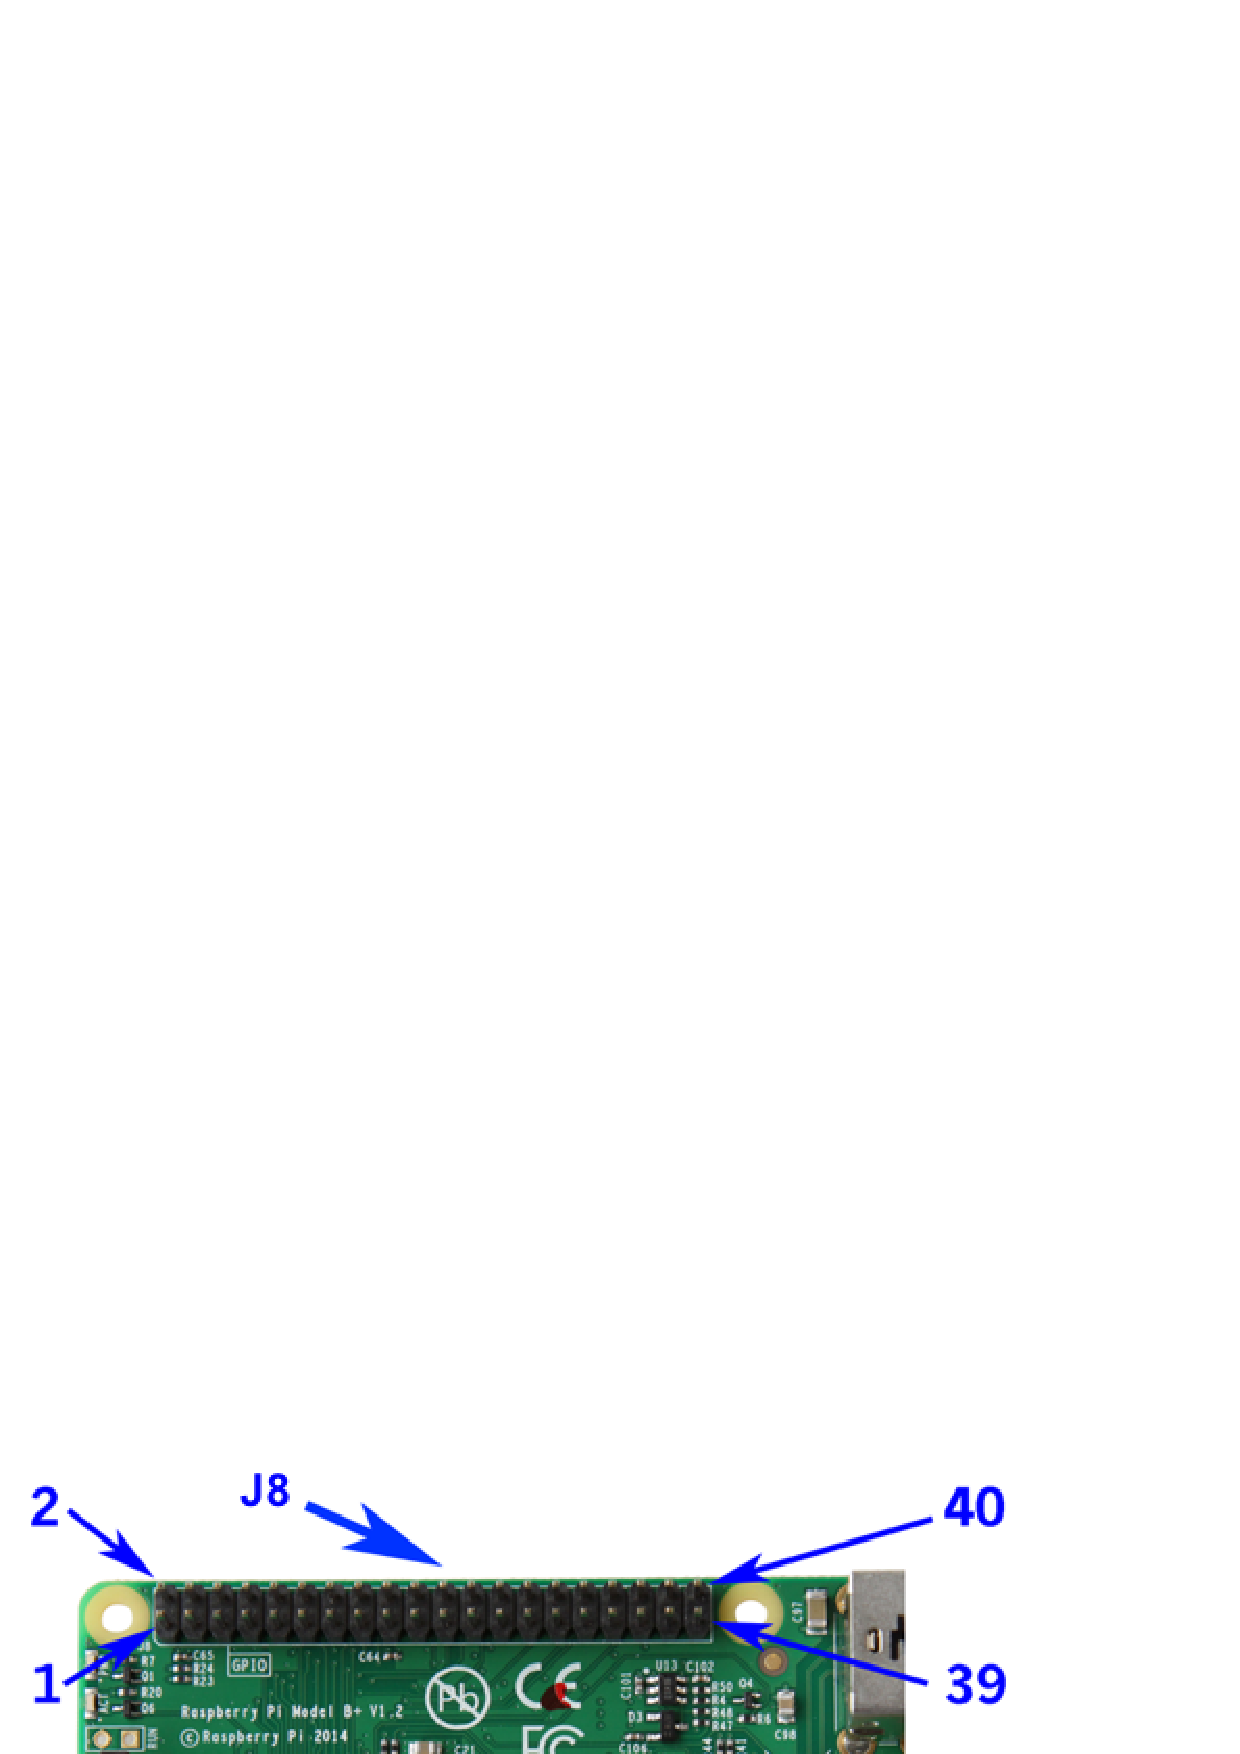
\includegraphics[width=\columnwidth]{./figs/gpio2}
\end{center}
\captionof{figure}{GPIO pin snapshot on Pi.}
\label{fig_1_3a}	
\end{figure}
%
\begin{figure}
\begin{center}
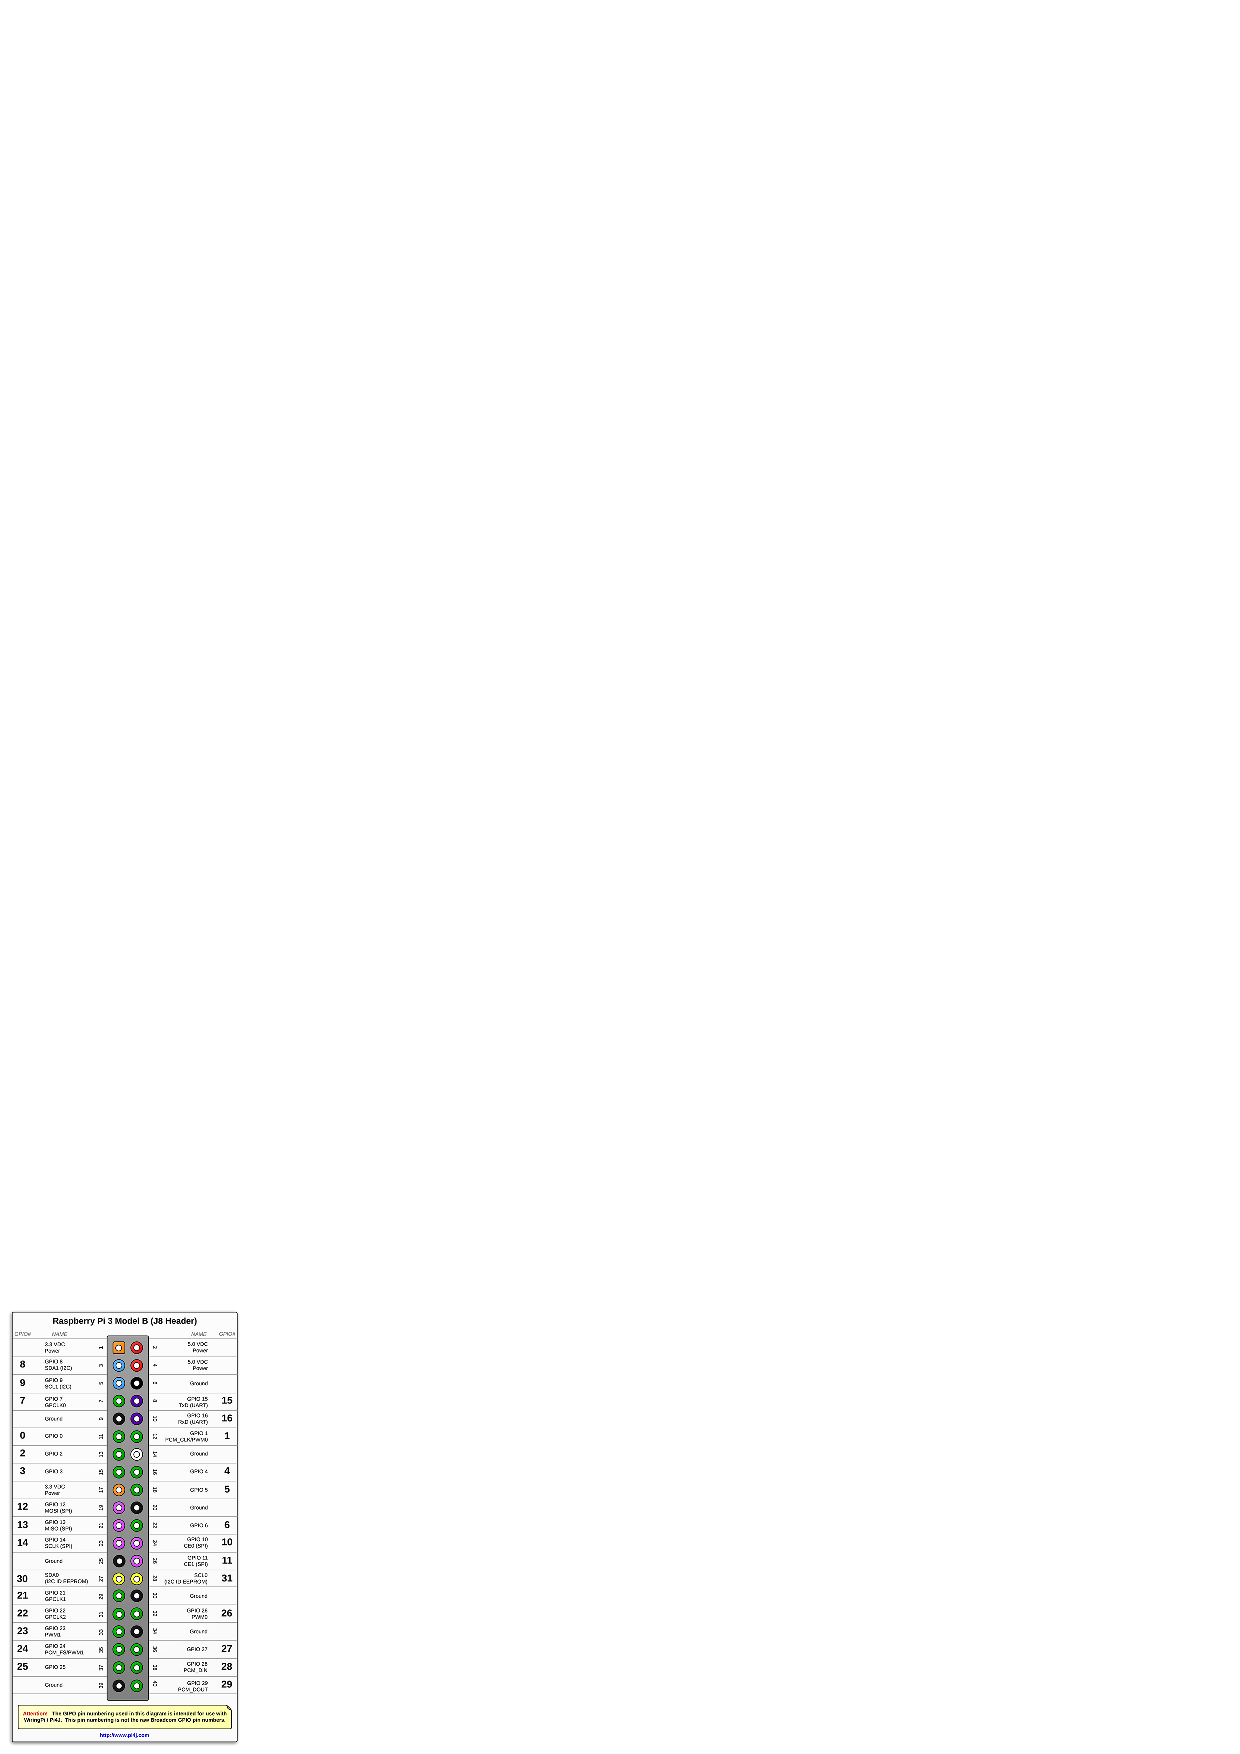
\includegraphics[width=\columnwidth]{./figs/gpio1}
\end{center}
\captionof{figure}{GPIO Wiring Pi pin configuration.}
\label{fig_1_3b}	
\end{figure}
\renewcommand{\thefigure}{\theproblem}
\begin{problem}
Connect the a-g pins of the display to the GPIO pins 0-6 of the Pi shown in \ref{fig_1_3a} and \ref{fig_1_3b}.
\end{problem}
\begin{problem}
Type the following C code and excute. What do you observe?
\end{problem}
\solution
\lstinputlisting[language=C]{./code/seven_seg_disp.c}
\begin{problem}
Now generate the numbers 0-9 by modifying the above program.
\end{problem}
\begin{problem}
Suitably modify the above program to obtain a decade counter.
\end{problem}


%\begin{problem}
%\label{prob:first_code}
%%Type the following code and execute. What do you observe?
%%\lstinputlisting[language=C]{./codes/bcd_seven.c}
%%// the setup function runs once when you press reset or power the board
int a=1,b=0,c=0,d=1,e=1,f=1,g=1;
void setup() {
    pinMode(2, OUTPUT);  
    pinMode(3, OUTPUT);
    pinMode(4, OUTPUT);
    pinMode(5, OUTPUT);
    pinMode(6, OUTPUT);
    pinMode(7, OUTPUT);
    pinMode(8, OUTPUT);            
}

// the loop function runs over and over again forever
void loop() {
  
  digitalWrite(2, a); 
  digitalWrite(3, b); 
  digitalWrite(4, c); 
  digitalWrite(5, d); 
  digitalWrite(6, e); 
  digitalWrite(7, f);     
  digitalWrite(8, g); 
}


%\end{problem}
%\begin{problem}
%Now generate the numbers 0-9 by modifying the above program.
%\end{problem}
%%
%%\newpage

%%\section{Combinational Logic}
%%
%\subsection{Counting Decoder}
	%In the  truth table in Table \ref{table:counter_decoder},  $W,X,Y,Z$ are the inputs
%and $A,B,C,D$ are the outputs. This table represents the system that increments the numbers 0-8 by 1 and resets the number 9 to 0
%%
%Note that  $D = 1$ for the inputs $0111$ and $1000$.  Using {\em boolean} logic,
%%
%\begin{equation}
%\label{bool_logic}
%D = WXYZ^{'} + W^{'}X^{'}Y^{'}Z
%\end{equation}
%%
%Note that $0111$ results in the expression $WXYZ^{'}$ and $1000$ yields $W^{'}X^{'}Y^{'}Z$. 
%%The $\&\&$ operand is used for the boolean AND (multiplication) operation, the $||$ operand is used for the OR (addition) operation and the ! operand is used for the NOT ($^{'}$) operation in Arduino code.  For example, the expression for \eqref{bool_logic} in Arudino is
%%\begin{verbatim}
%%D = (W&&X&&Y&&!Z)||(!W&&!X&&!Y&&Z);
%%\end{verbatim}

%\begin{problem}
	%\label{counter_dec}

%Write the boolean logic functions for $A,B,C$ in terms of $W,X,Y,Z$.
%\end{problem}
%%
%\input{./figs/counter_decoder}
%%
%%
%\begin{problem}
%%	\label{D_code}
%Write a program for implementing Table \ref{counter_dec}.
%%\eqref{bool_logic} in Arduino.
%\end{problem}
%%
%\solution
%%\lstinputlisting[language=C]{./codes/count_decoder.c}
%%
%%\begin{problem}
%%Modify the above program by keeping W=0,X=0,Y=0,Z=1 and A=1 and execute.  Verify that your results are consistent with Table \ref{counter_dec}.
%%\end{problem}

%\begin{problem}
%Verify if your logic is correct by observing the output on the seven segment display for different inputs.
%\end{problem}
%%
%\begin{problem}
%Connect GPIO pin 10 to the dot pin of the display and execute the following code.
%\end{problem}
%%\lstinputlisting[language=C]{./codes/blink.c}
%%
%%
%\begin{problem}
%A decade counter counts the numbers from 0-9 and then resets to 0.  Suitable modify the above programs to obtain a decade counter.
%\end{problem}

%\subsection{Display Decoder}
%%
%\begin{problem}
%Now write the truth table for the seven segment display decoder (IC 7447).  The inputs will be $A,B,C,D$ and the outputs will be $a,b,c,d,e,f,g$.
%\end{problem}
%%
%\begin{problem}
%\label{seven_seg_disp_logic}
%Obtain the logic functions for outputs $a,b,c,d,e,f,g$ in terms of the inputs $A,B,C,D$.
%\end{problem}
%\begin{problem}
%Disconnect the Pi from IC 7447 and connect the pins GPIO 0-6 in the Pi directly to the seven segment display.
%\end{problem}
%\begin{problem}
%Write a new program to implement the logic in Problem \ref{seven_seg_disp_logic} and observe the output in the display.  You have designed the logic for IC 7447!
%\end{problem}
%\begin{problem}
%Now include your counting decoder program in the  display decoder program
%and see if the display shows the consecutive number.
%\end{problem}
%A decade counter counts the numbers from 0-9 and then resets to 0.
%\begin{problem}
%Suitably modify the above program to obtain a decade counter.
%\end{problem}




%\begin{problem}
%Generate the boolean functions for the segments $a-f$ using the table in Problem \ref{bcd_ss}.  For example, the function for $a$ is obtained from the table as
%\begin{equation}
%a=\bar{D}\bar{C}\bar{B}A+\bar{D}C\bar{B}\bar{A}
%\label{boolean}
%\end{equation}
%\end{problem}
%%
%\begin{problem}
	%\label{counter_dec}
%Write functions for $A,B,C,D$ in Arduino using the following table and verify using the Arduino driven display.
		%\input{counter_decoder}
%\end{problem}
%\begin{problem}
	%Write a module for decimal to binary conversion
	%according to the example given below
	%\input{conversion}
	%%
	%$N \% 2$ gives the remainder and $N/2$ gives the quotient
%	and use it in the above code so that decimal values are given as input in the program and observed as output in the display. Note that the following code
%	\begin{verbatim}
%	a % b
%	\end{verbatim}
%	can be used to obtain the remainder when a is divided by b and
%	\begin{verbatim}
%	a/b
%	\end{verbatim}
%	gives the quotient.
%\end{problem}
 
%
%\newpage
%\section{$M$-ary Modulation}
%\subsection{Angle Bisectors}

\begin{figure}[!h]
	\begin{center}
		
		%
\includegraphics[width=\columnwidth]{./figs/ch3_angle_bisector}
		%\vspace*{-10cm}
		\resizebox{\columnwidth}{!}{\begin{tikzpicture}
[scale=2,>=stealth,point/.style={draw,circle,fill = black,inner sep=0.5pt},]

\node (D) at (0, 0)[point,label=below :$D$] {};
\node (A) at (0, 3)[point,label=above :$A$]{};
\node (B) at (-3, 0)[point,label=below left:$B$]{};
\node (C) at (3, 0)[point,label=below right:$C$]{};
\node (O) at (0, 1.3)[point,label=below right:$O$]{};
\node (F) at (-1.1, 1.9)[point,label=above left:$F$]{};
\node (E) at (1.1, 1.9)[point,label=above right:$E$]{};

\draw (D)--(B);
\draw (B)--(A);
\draw (A)--(C);
\draw (C)--(D);
\draw [thick,dashed] (A) -- (D);
\draw [thick,dashed] (O) -- (E);
\draw [thick,dashed] (O) -- (F);
\draw (B)--(O);
\draw (C)--(O);

\tkzMarkRightAngle[size=.2](A,D,C)
\tkzMarkRightAngle[size=.15](B,F,O);
\tkzMarkRightAngle[size=.15](C,E,O);
\tkzMarkAngle[size=.4](D,B,O);
\tkzMarkAngle[size=.35](O,B,F);
\tkzMarkAngle[size=.54](E,C,O);
\tkzMarkAngle[size=.5](E,C,O);
\tkzMarkAngle[size=.6](O,C,D);
\tkzMarkAngle[size=.65](O,C,D);

\end{tikzpicture}}
	\end{center}
	\caption{Angle bisectors meet at a point}
	\label{ch3_angle_bisector}	
\end{figure}

\begin{definition}
	In Fig. \ref{ch3_angle_bisector}, $OB$ divides the  $\angle B$ into half, i.e.\begin{equation}
	\angle OBC = \angle OBA
	\end{equation}
	$OB$ is known as an angle bisector.
\end{definition}
	$OB$ and $OC$ are angle bisectors of angles $B$ and $C$. $OA$ is joined and $OD, OF$ and $OE$ are perpendiculars to sides $a,b$ and $c$.
\begin{problem}
  Show that $OD = OE = OF$.
\end{problem}
\proof In $\Delta$s $ODC$ and $OEC$,
\begin{align}
OD &= OC \sin \frac{C}{2}
\\
OE &= OC \sin \frac{C}{2} 
\\
\Rightarrow OD &=OE.
\end{align}
Similarly,
\begin{equation}
OD = OF.
\end{equation}
%
\begin{problem}
	Show that OA is the angle bisector of $\angle A$
\end{problem}
\proof In $\Delta$s $OFA$ and $OEA$,
\begin{align}
OF &= OE
\\
\Rightarrow OA \sin OAF &= OA \sin OAE \\
\Rightarrow \sin OAF &=  \sin OAE \\
\Rightarrow \angle OAF &= \angle OAE
\end{align}
which proves that $OA$ bisects $\angle A$.
{\em Conclusion:} The angle bisectors of a triangle meet at a point.


\subsection{Congruent Triangles}
%
\begin{problem}
	Show that in $\Delta$s $ODC$ and $OEC$, corresponding sides and angles are equal.
\end{problem}
\begin{definition}
	Note that    $\Delta$s $ODC$ and $OEC$ are known as congruent triangles.  To show that two triangles are congruent, it is sufficient to show that some angles and sides are equal.
\end{definition}
\begin{problem}
SSS:	Show that if the corresponding sides of three triangles are equal, the triangles are congruent.
\end{problem}
\begin{problem}
ASA:	Show that if two angles and any one side  are equal in corresponding triangles, the triangles are congruent.
\end{problem}
\begin{problem}
SAS:	Show that if two sides and the angle between them are equal in corresponding triangles, the triangles are congruent.
\end{problem}
\begin{problem}
RHS:	For two right angled triangles, if the hypotenuse and one of the sides are equal, show that the triangles are congruent.
\end{problem}
	%
%%
\subsection{Perpendicular Bisectors}
\begin{definition}
	In Fig. \ref{ch3_perp_bisector}, OD $\perp BC$ and $BD=DC$. $OD$ is defined as the perpendicular bisector of $BC$.
\end{definition}

\begin{problem}
	In Fig. \ref{ch3_perp_bisector}, show that $OA=OB=OC$.
\end{problem}
%%
%%
\begin{figure}[!h]
	\begin{center}
		
		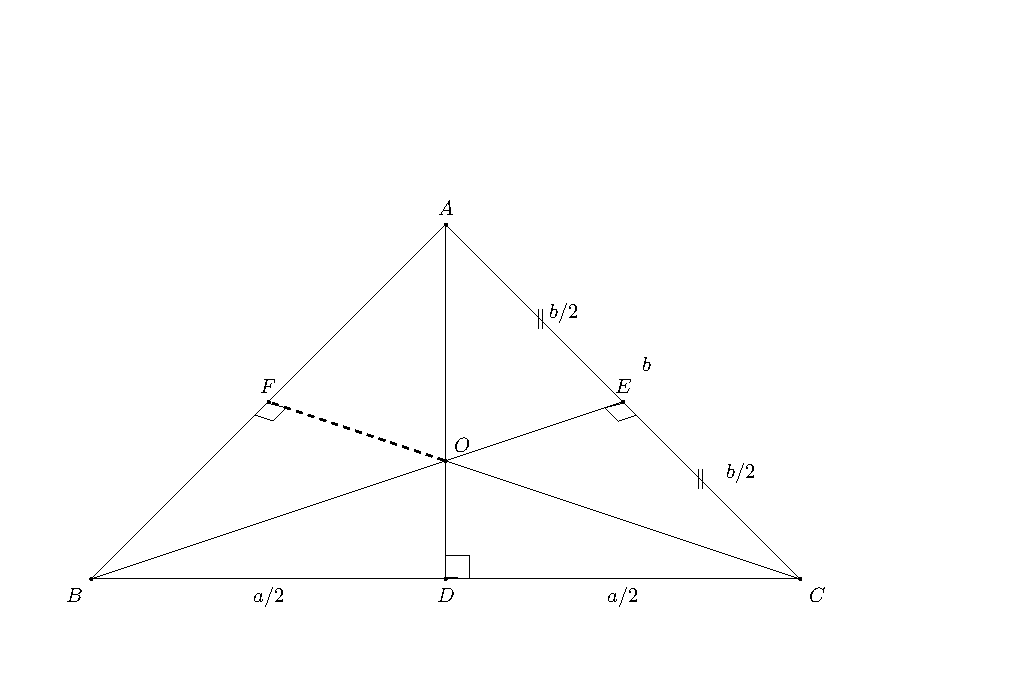
\includegraphics[width=\columnwidth]{./figs/fig_3.8.eps}
%		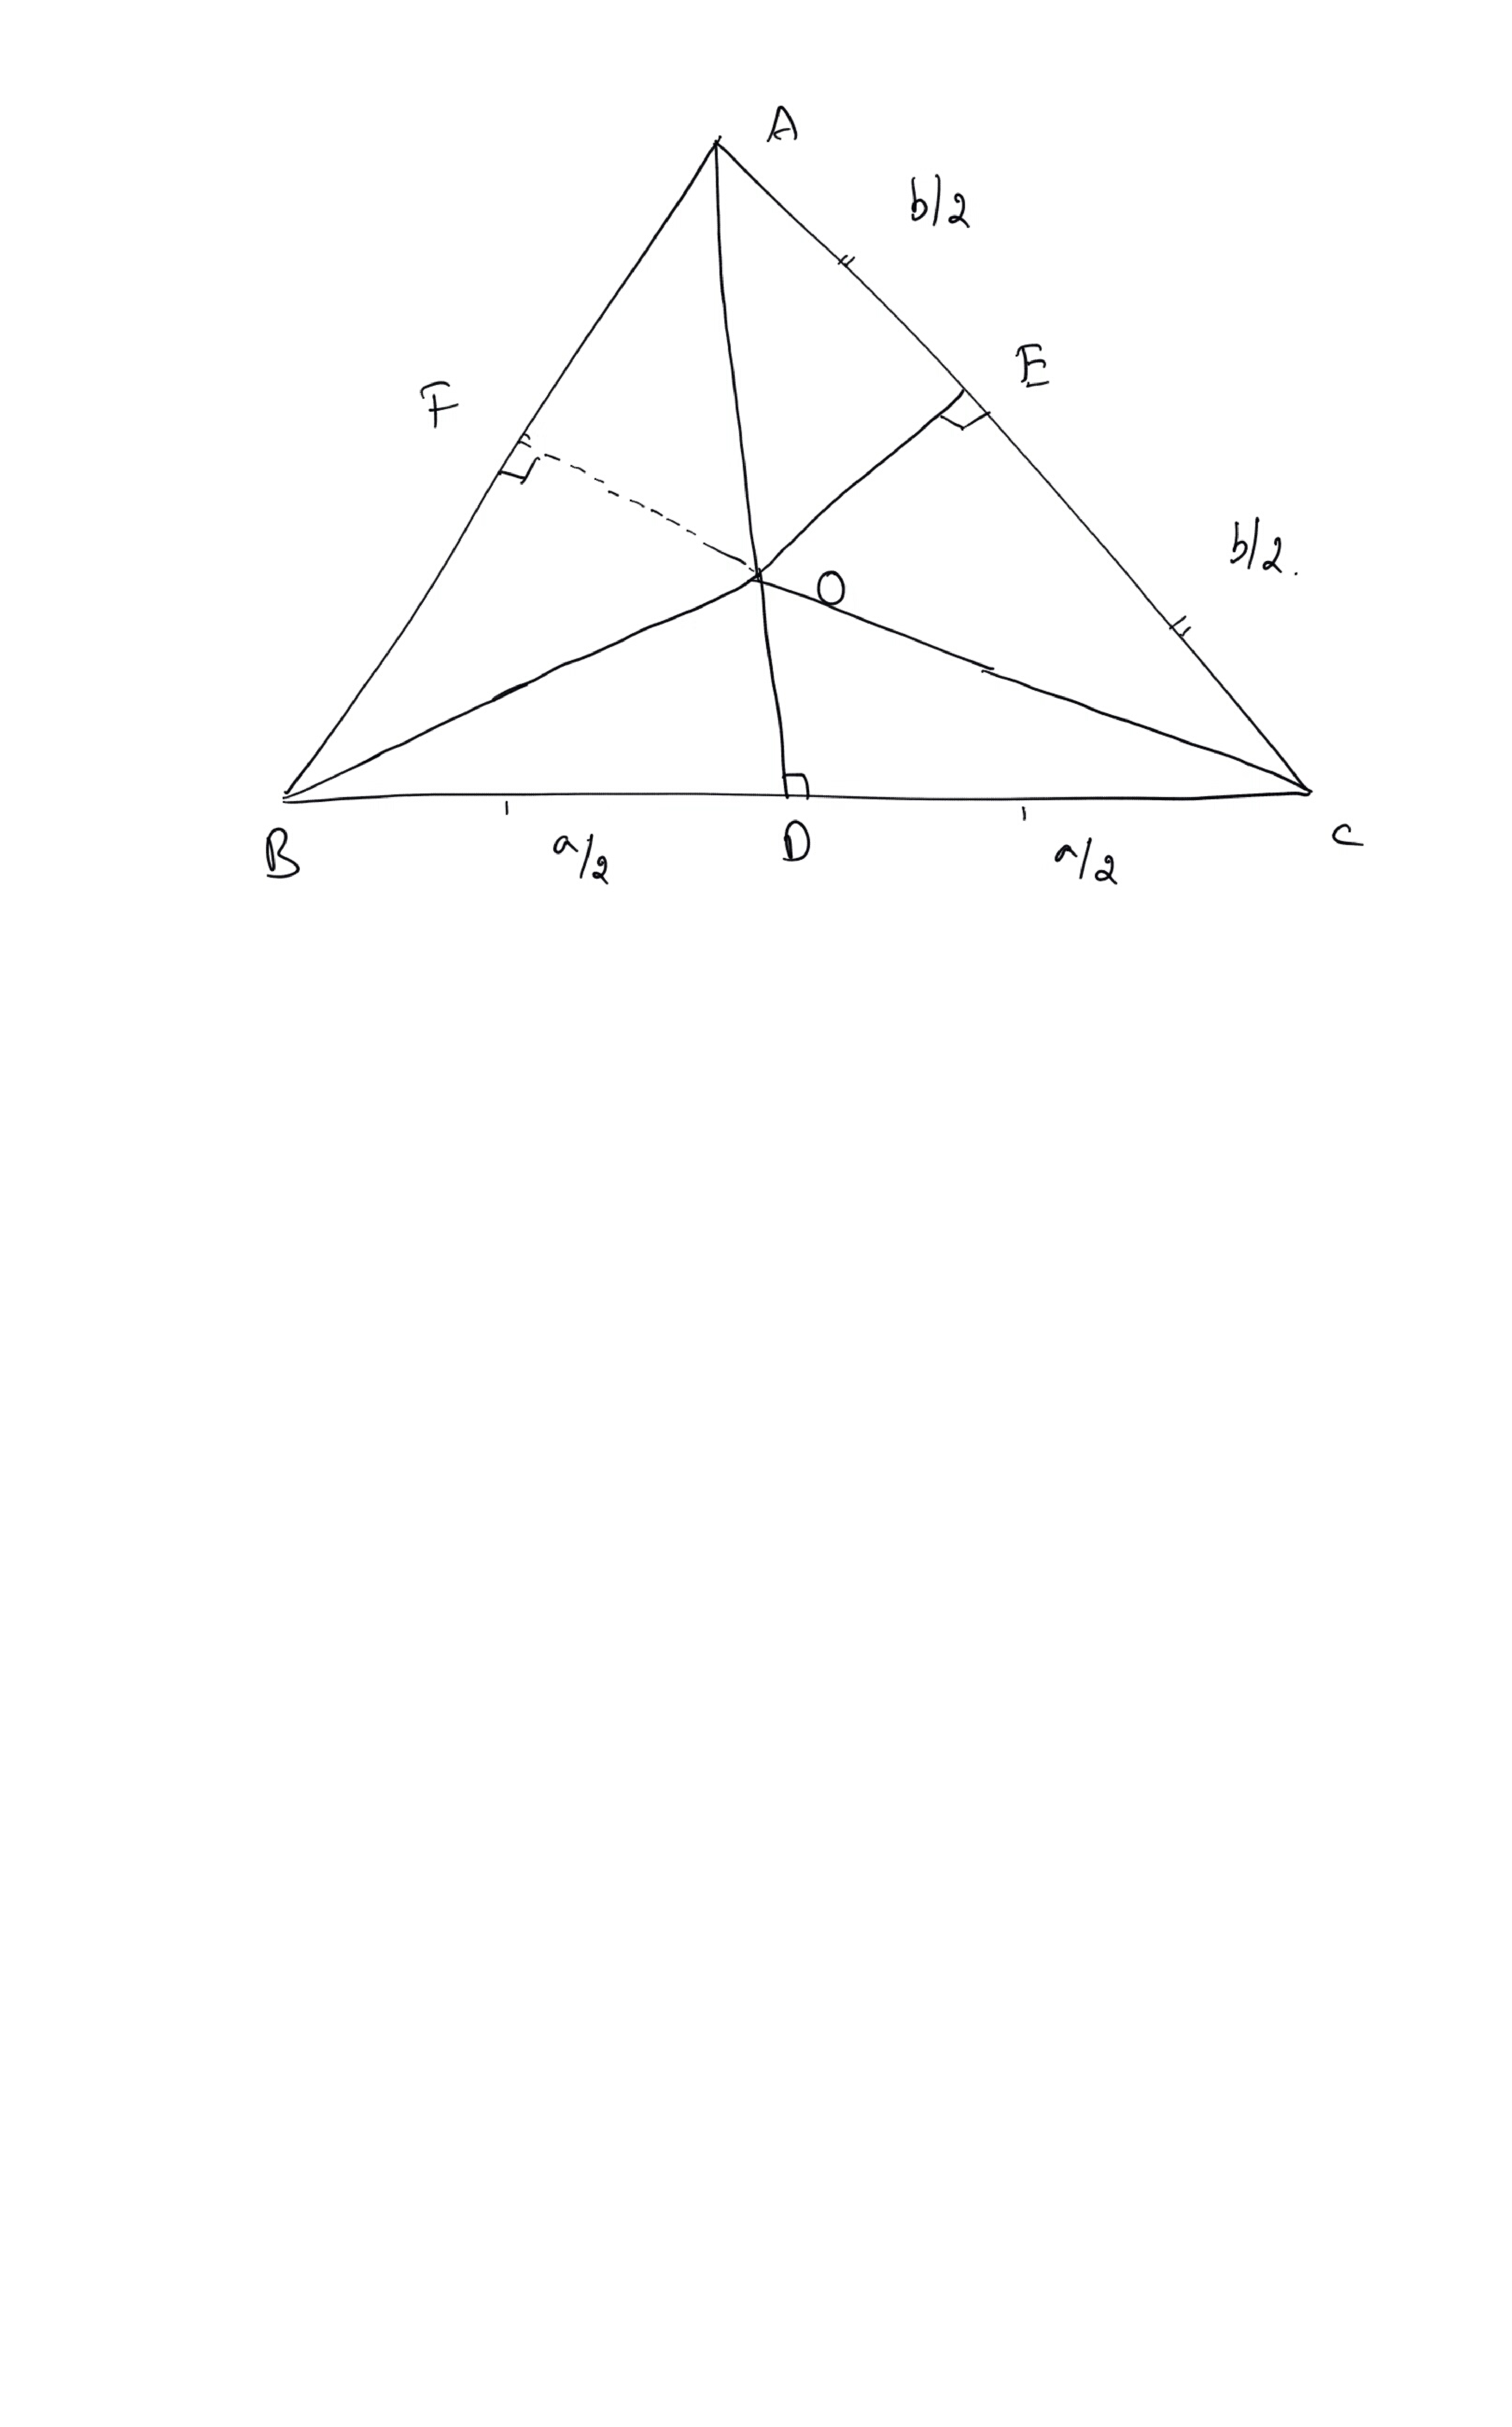
\includegraphics[width=\columnwidth]{./figs/ch3_perp_bisector}
		%\vspace*{-10cm}
%		\resizebox{\columnwidth}{!}{\documentclass{standalone}
\usepackage{tikz}
\usepackage{tkz-euclide}
\usetkzobj{all}
%\usepackage{amsmath}
\providecommand{\brak}[1]{\ensuremath{\left(#1\right)}}

\begin{document}
\begin{tikzpicture}
[scale=2,>=stealth,point/.style={draw,circle,fill = black,inner sep=0.5pt},]

\node (E) at (1.5, 1.5)[point,label=above :$E$] {};
\node (F) at (-1.5, 1.5)[point,label=above :$F$] {};
\node (A) at (0, 3)[point,label=above :$A$]{};
\node (B) at (-3, 0)[point,label=below left:$B$]{};
\node (C) at (3, 0)[point,label=below right:$C$]{};
\node (D) at (0,0)[point,label=below :$D$] {};
\node (O) at (0,1)[point,label=above right :$O$] {};


\draw (B)--(A);
\draw (A)--(C);
\draw (B)--(C);
\draw (B)--(E);
\draw (C)--(O);
\draw (A)--(D);
\draw [thick,dashed] (O) -- (F);

\node [above] at (1.7,1.7) {$b$};
\node [above] at (2.5,.75) {$b/2$};
\node [above] at (1,2.1) {$b/2$};
\node [above] at (-1.5,-0.3){$a/2$};
\node [above] at (1.5,-0.3){$a/2$};
\tkzMarkRightAngle[size=.16](B,F,O)
\tkzMarkRightAngle[size=.16](C,E,O)
\tkzMarkRightAngle[size=.2](A,D,C)
\draw   -- (4.3,1.7) node[midway] {$\parallel$};
\draw   -- (1.6,4.4) node[midway] {$\parallel$};

\end{tikzpicture}
\end{document}}
	\end{center}
	\caption{Perpendicular bisectors meet at a point}
	\label{ch3_perp_bisector}	
\end{figure}
%
\proof In $\Delta$s $ODB$ and $ODC$, using Budhayana's theorem,
%
\begin{equation}
\begin{split}
OB^2 &= OD^2 + BD^2 \\
OC^2 &= OD^2 + DC^2 
\end{split}
\end{equation}
%
Since $BD = DC = \frac{a}{2}$, $OB = OC$.  Similarly, it can be shown that $OA = OC$.  Thus, $OA=OB=OC$.
%
\begin{definition}
	In $\Delta AOB$, $OA = OB$.  Such a triangle is known as an isoceles triangle.
\end{definition}
%
\begin{problem}
	Show that $AF = BF$.
\end{problem}
\proof Trivial using Budhayana's theorem.  This shows that $OF$ is a perpendicular bisector of $AB$. 
{\em Conclusion:}  The perpendicular bisectors of a triangle meet at a point.
%
\subsection{Perpendiculars from Vertex to Opposite Side}
	%
	%
	In Fig. \ref{ch3_perp_triang}, $AD \perp BC$ and $BE \perp AC$. $CF$ passes through $O$ and meets
	$AB$ at $F$.  	
\begin{problem}
	Show that 
	\begin{align}
	OE = c \cos A \cot C
	\end{align}
\end{problem}
	\begin{figure}[!h]
		\begin{center}
			
			%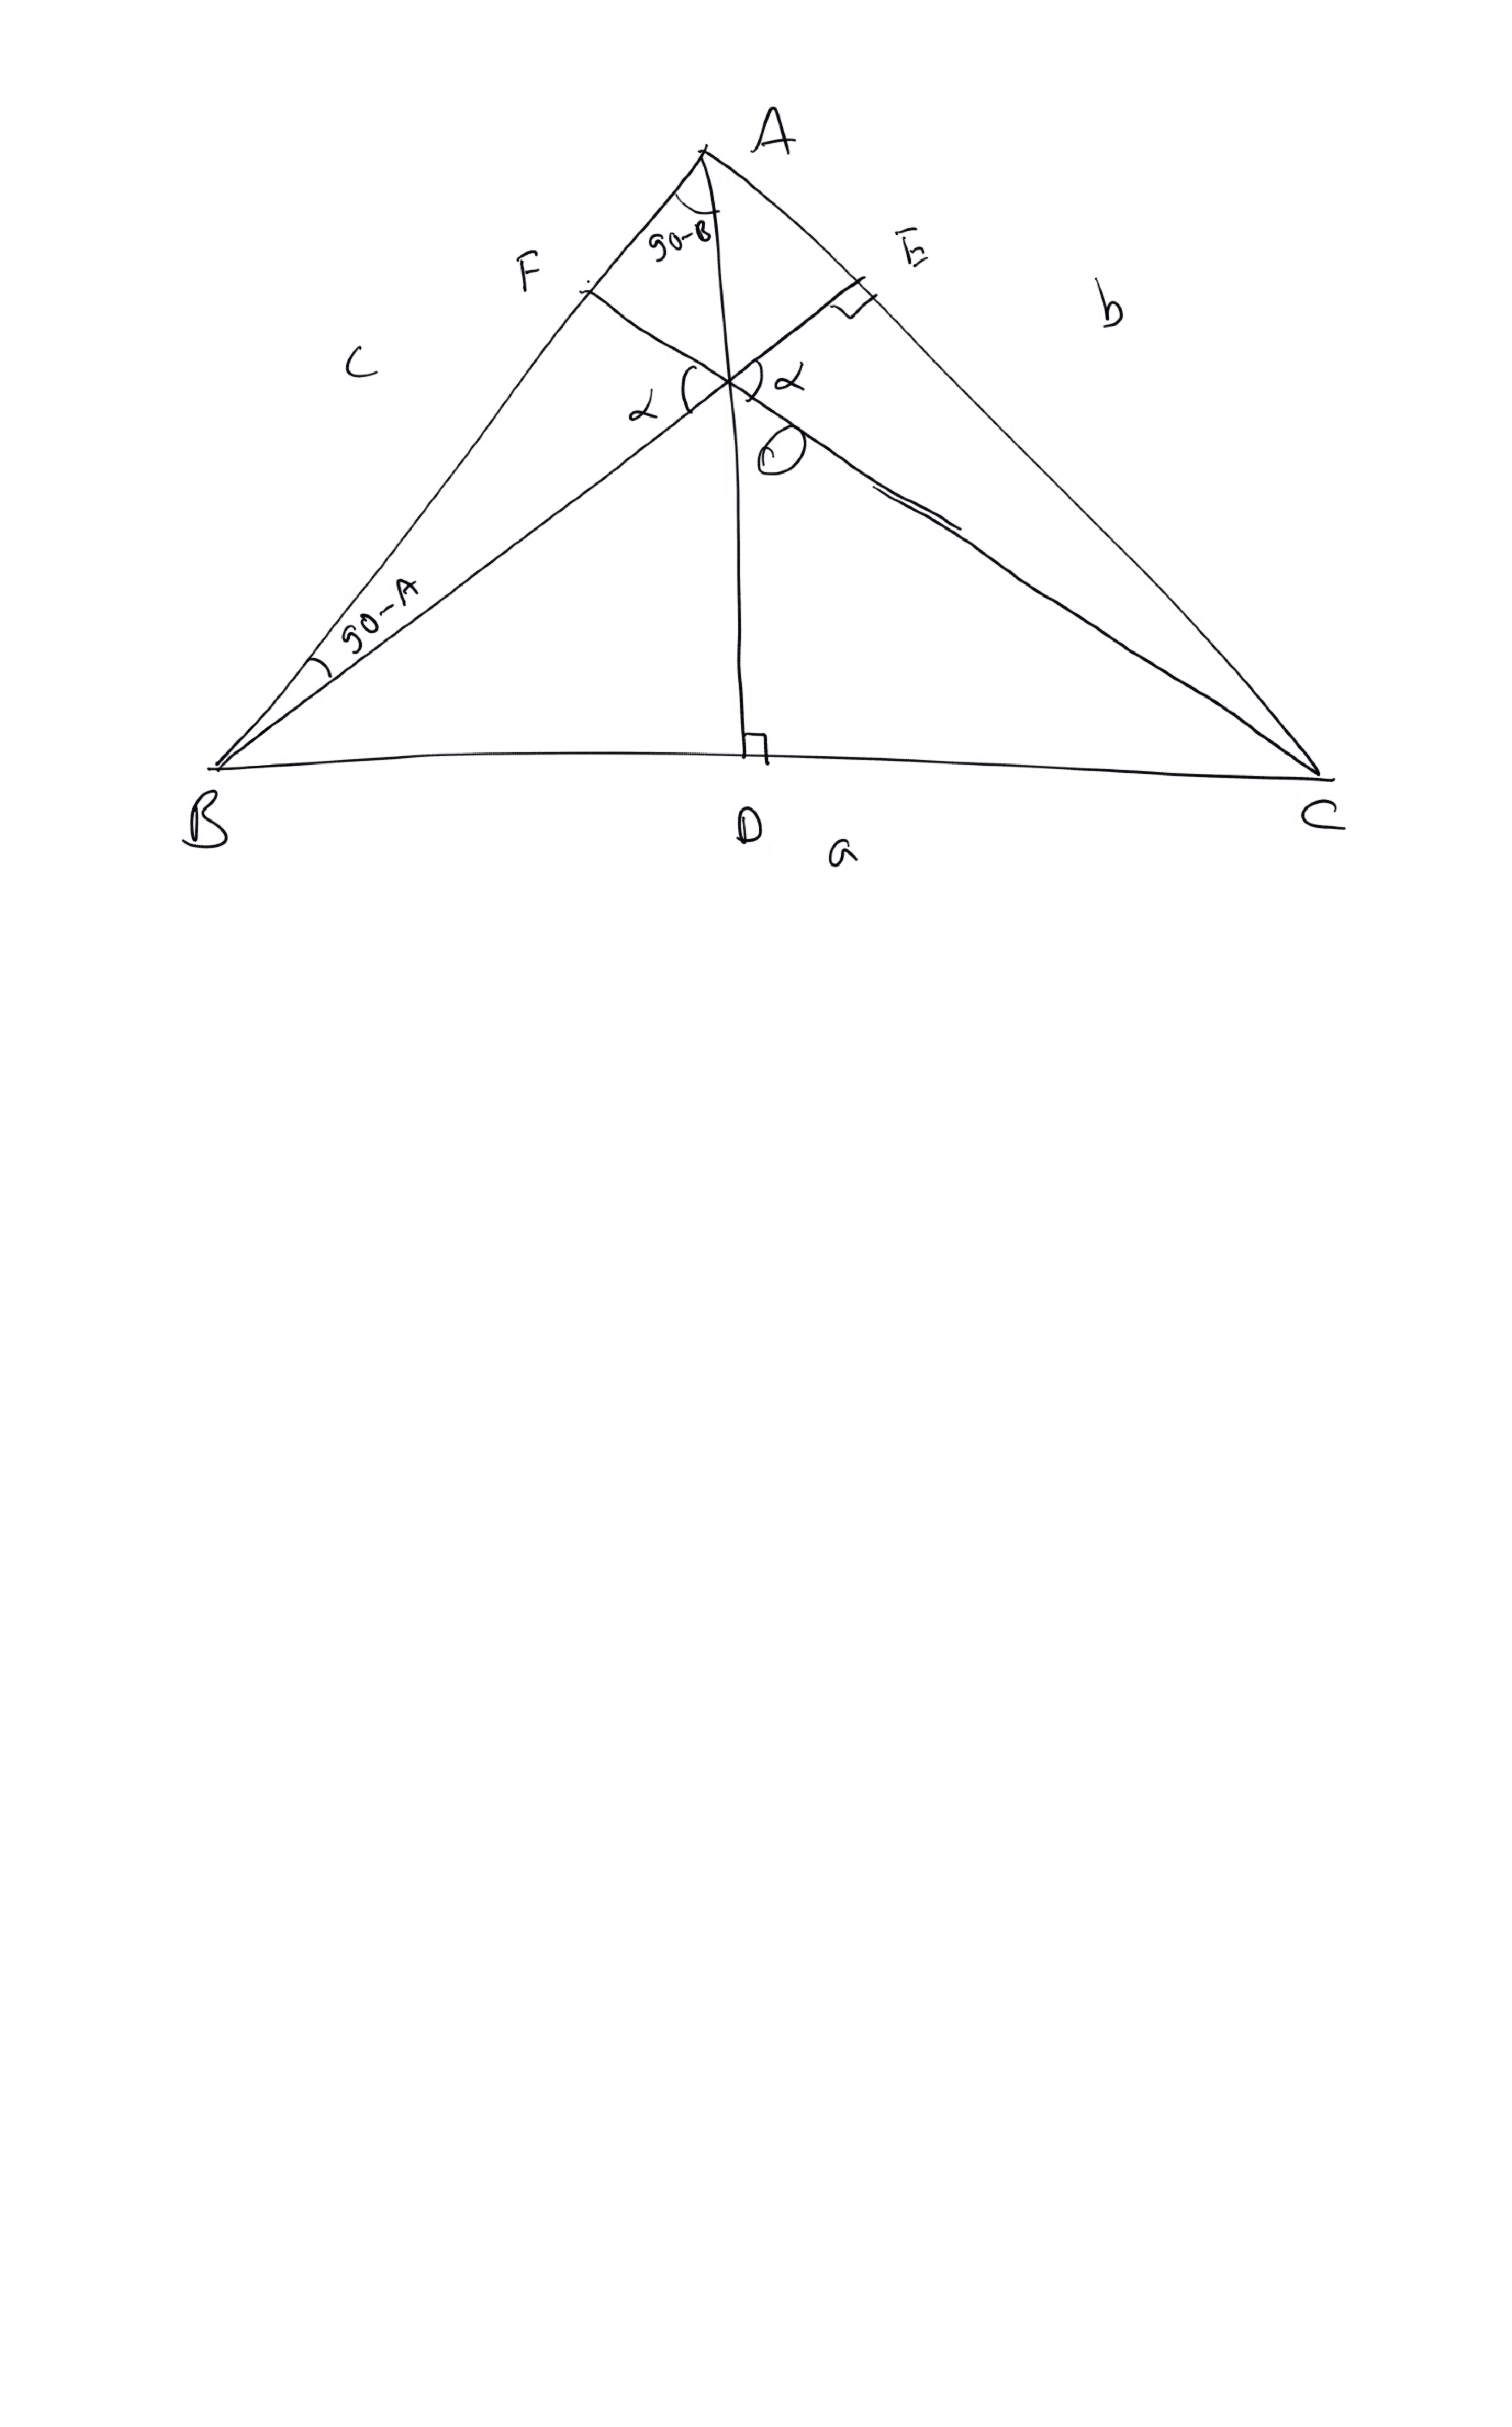
\includegraphics[width=\columnwidth]{./figs/ch3_perp_triang}
			%\vspace*{-10cm}
			\resizebox{\columnwidth}{!}{\begin{tikzpicture}
[scale=2,>=stealth,point/.style={draw,circle,fill = black,inner sep=0.5pt},]

\node (E) at (1.5, 1.5)[point,label=above :$E$] {};
\node (F) at (-1.5, 1.5)[point,label=above :$F$] {};
\node (A) at (0, 3)[point,label=above :$A$]{};
\node (B) at (-3, 0)[point,label=below left:$B$]{};
\node (C) at (3, 0)[point,label=below right:$C$]{};
\node (O) at (0,1)[point,label=above right :$O$] {};
\node (D) at (0,0)[point,label=below :$D$] {};


\draw (B)--(A);
\draw (A)--(C);
\draw (B)--(E);
\draw (C)--(F);
\draw (B)--(C);
\draw (A)--(D);

\node [below] at (0,-0.3) {$a$};
\node [above] at (-1.7,1.7) {$c$};
\node [above] at (1.7,1.7) {$b$};
\node [above] at (1,1.3) {$p$};
\node [above] at (-1,1.3) {$q$};
\node [above] at (-2.3,0.24){\rotatebox{45}{$90-A$}};
\node [above] at (-0.4,2.1) {\rotatebox{45}{$90-B$}};
\node [above] at (0.4,2.1) {\rotatebox{-45}{$90-C$}};

\tkzMarkAngle[size=.3](F,O,B);
\tkzMarkAngle[size=.3](C,O,E);
\tkzMarkAngle[size=.4](O,B,F);
\tkzMarkAngle[size=.2](F,A,O);
\tkzMarkAngle[size=.3](O,A,E);
\draw (-0.5,1) node{$\alpha$};
\draw (0.5,1) node{$\alpha$};

\end{tikzpicture}
}
		\end{center}
		\caption{Perpendiculars from vertex to opposite side meet at a point}
		\label{ch3_perp_triang}	
	\end{figure}
%
\proof In $\Delta$ s $AEB$ and $AEO$,
%
\begin{align}
AE &= c \cos A \\
OE &= AE \tan \brak{90^{\degree} - C} \brak{\because ADC \text{ is right angled}} \\
&= AE \cot C
\end{align}
%
From both the above, we get the desired result.
%
\begin{problem}
	Show that $\alpha = A$.
\end{problem}
\proof In $\Delta OEC$,
%
\begin{equation}
CE = a \cos C \brak{\because BEC \text{ is right angled}}
\end{equation}
%
Hence,
%
\begin{equation}
\begin{split}
\tan \alpha &= \frac{CE}{OE} \\
&=  \frac{a \cos C}{c \cos A \cot C} \\
&=  \frac{a \cos C \sin C}{c \cos A \cos C} \\
&= \frac{a \sin C}{c \cos A } \\
&= \frac{c \sin A}{c \cos A } \brak{\because \frac{a}{\sin A} = \frac{c}{\sin C}}\\
&= \tan A\\
\Rightarrow \alpha = A
\end{split}
\end{equation}
%
\begin{problem}
	Show that $CF \perp AB$
\end{problem}
\proof Consider triangle OFB and the result of the previous problem.  $\because$ the sum of the angles of a triangle is $180^{\degree}$, $\angle CFB = 90^{\degree}$.
{\em Conclusion: The perperdiculars from the vertex of a triangle to the opposite side meet at a point.} 

%\newpage
%\section{BER in Rayleigh Flat Slowly Fading Channels}
%\subsection{Chord of a Circle}

\begin{figure}[!h]
	\begin{center}
		
		
\includegraphics[width=\columnwidth]{./figs/ch4_circle_def}
		\vspace*{-10cm}
	\end{center}
	\caption{Circle Definitions}
	\label{ch4_circle_def}	
\end{figure}
\begin{definition}
	Fig. \ref{ch4_circle_def} represents a circle.  The points in the circle are at a distance $r$ from the centre $O$.  $r$ is known as the radius.
\end{definition}

\subsection{Chords of a circle}
\begin{definition}
	In Fig. \ref{ch4_circle_def}, $A$ and $B$ are points on the circle.  The line $AB$ is known as a chord of the circle.
\end{definition}
%
%
\begin{problem}
	\label{ch4_prob_circle_subtend}
	In Fig. \ref{ch4_circle_subtend}  Show that $\angle OAB = 2\angle APB $.
\end{problem}
\begin{figure}[!h]
	\begin{center}
		
		
\includegraphics[width=\columnwidth]{./figs/ch4_circle_subtend}
		\vspace*{-10cm}
	\end{center}
	\caption{Angle subtended by chord $AB$ at the centre $O$ is twice the angle subtended at $P$. }
	\label{ch4_circle_subtend}	
\end{figure}

\proof In Fig. \ref{ch4_circle_subtend}, the triangeles $OPA$ and $OPB$ are isosceles. Hence,
%
\begin{align}
\angle OPB = \angle OBP &= \theta_1 \\
\angle OPA = \angle OAP &= \theta_2
\end{align}
%
Also, $\alpha$ and $\beta$ are exterior angles corresponding to the triangle $OPB$ and $OPA$ respectively. Hence
%
\begin{align}
\alpha &= 2\theta_1 \\
\beta &= 2\theta_2
\end{align}
%
Thus,
%
\begin{align}
\angle AOB &= \alpha + \beta \\
&= \theta_1 + \theta_2 \\
&= \angle APB
\end{align}
%
\begin{definition}
	The diameter of a circle is the chord that divides the circle into two equal parts. In Fig. \ref{ch4_circle_dia}, $AB$ is the diameter and passes through the centre $O$
\end{definition}
%
\begin{problem}
In Fig. \ref{ch4_circle_dia}, show that $\angle APB = 90^{\degree}$ .
\end{problem}
%
\begin{figure}[!h]
	\begin{center}
		
		
\includegraphics[width=\columnwidth]{./figs/ch4_circle_dia}
		\vspace*{-10cm}
	\end{center}
	\caption{Diameter of a circle.}
	\label{ch4_circle_dia}	
\end{figure}

\begin{problem}
	In Fig. \ref{ch4_chord_product}, show that 
	\begin{equation}
	\begin{split}
\angle ABD &= \angle ACD \\
\angle CAB &= \angle CDB	
	\end{split}
	\end{equation}
\end{problem}
\begin{figure}[!h]
	\begin{center}
		
		
\includegraphics[width=\columnwidth]{./figs/ch4_chord_product}
		\vspace*{-10cm}
	\end{center}
	\caption{$PA.PB = PC.PD$}
	\label{ch4_chord_product}	
\end{figure}
%
%
\proof Use Problem \ref{ch4_prob_circle_subtend}.
%
\begin{problem}
	In Fig. \ref{ch4_chord_product}, show that the triangles $PAB$ and $PBD$ are similar
\end{problem}
\proof Trivial using previous problem
\begin{problem}
	In Fig. \ref{ch4_chord_product}, show that 
	\begin{equation}
	PA.PB = PC.PD
	\end{equation}
\end{problem}
%
\proof Since triangles $PAC$ and $PBD$ are similar, 
%
\begin{align}
\frac{PA}{PD} &= \frac{PC}{PB} \\
\Rightarrow PA.PB &= PC.PD
\end{align}
%
%
\begin{definition}
	The line $PX$ in Fig. \ref{ch4_tangent_def} touches the circle at exactly one  point $P$. It is known as the tangent to the circle.
\end{definition}
%
%
\begin{problem}
	$OP$ is the perpendicular to the line $PX$ as shown in the Fig. \ref{ch4_short_dist}. Show that $OP$ is the shortest distance between the point $O$ and the line $PX$. 
\end{problem}
\proof Let $P_1$ be a point on the line $PX$. Then $OPP_1$ is a right angled triangle.  Using Budhayana's theorem,
%
\begin{figure}[!h]
	\begin{center}
		
		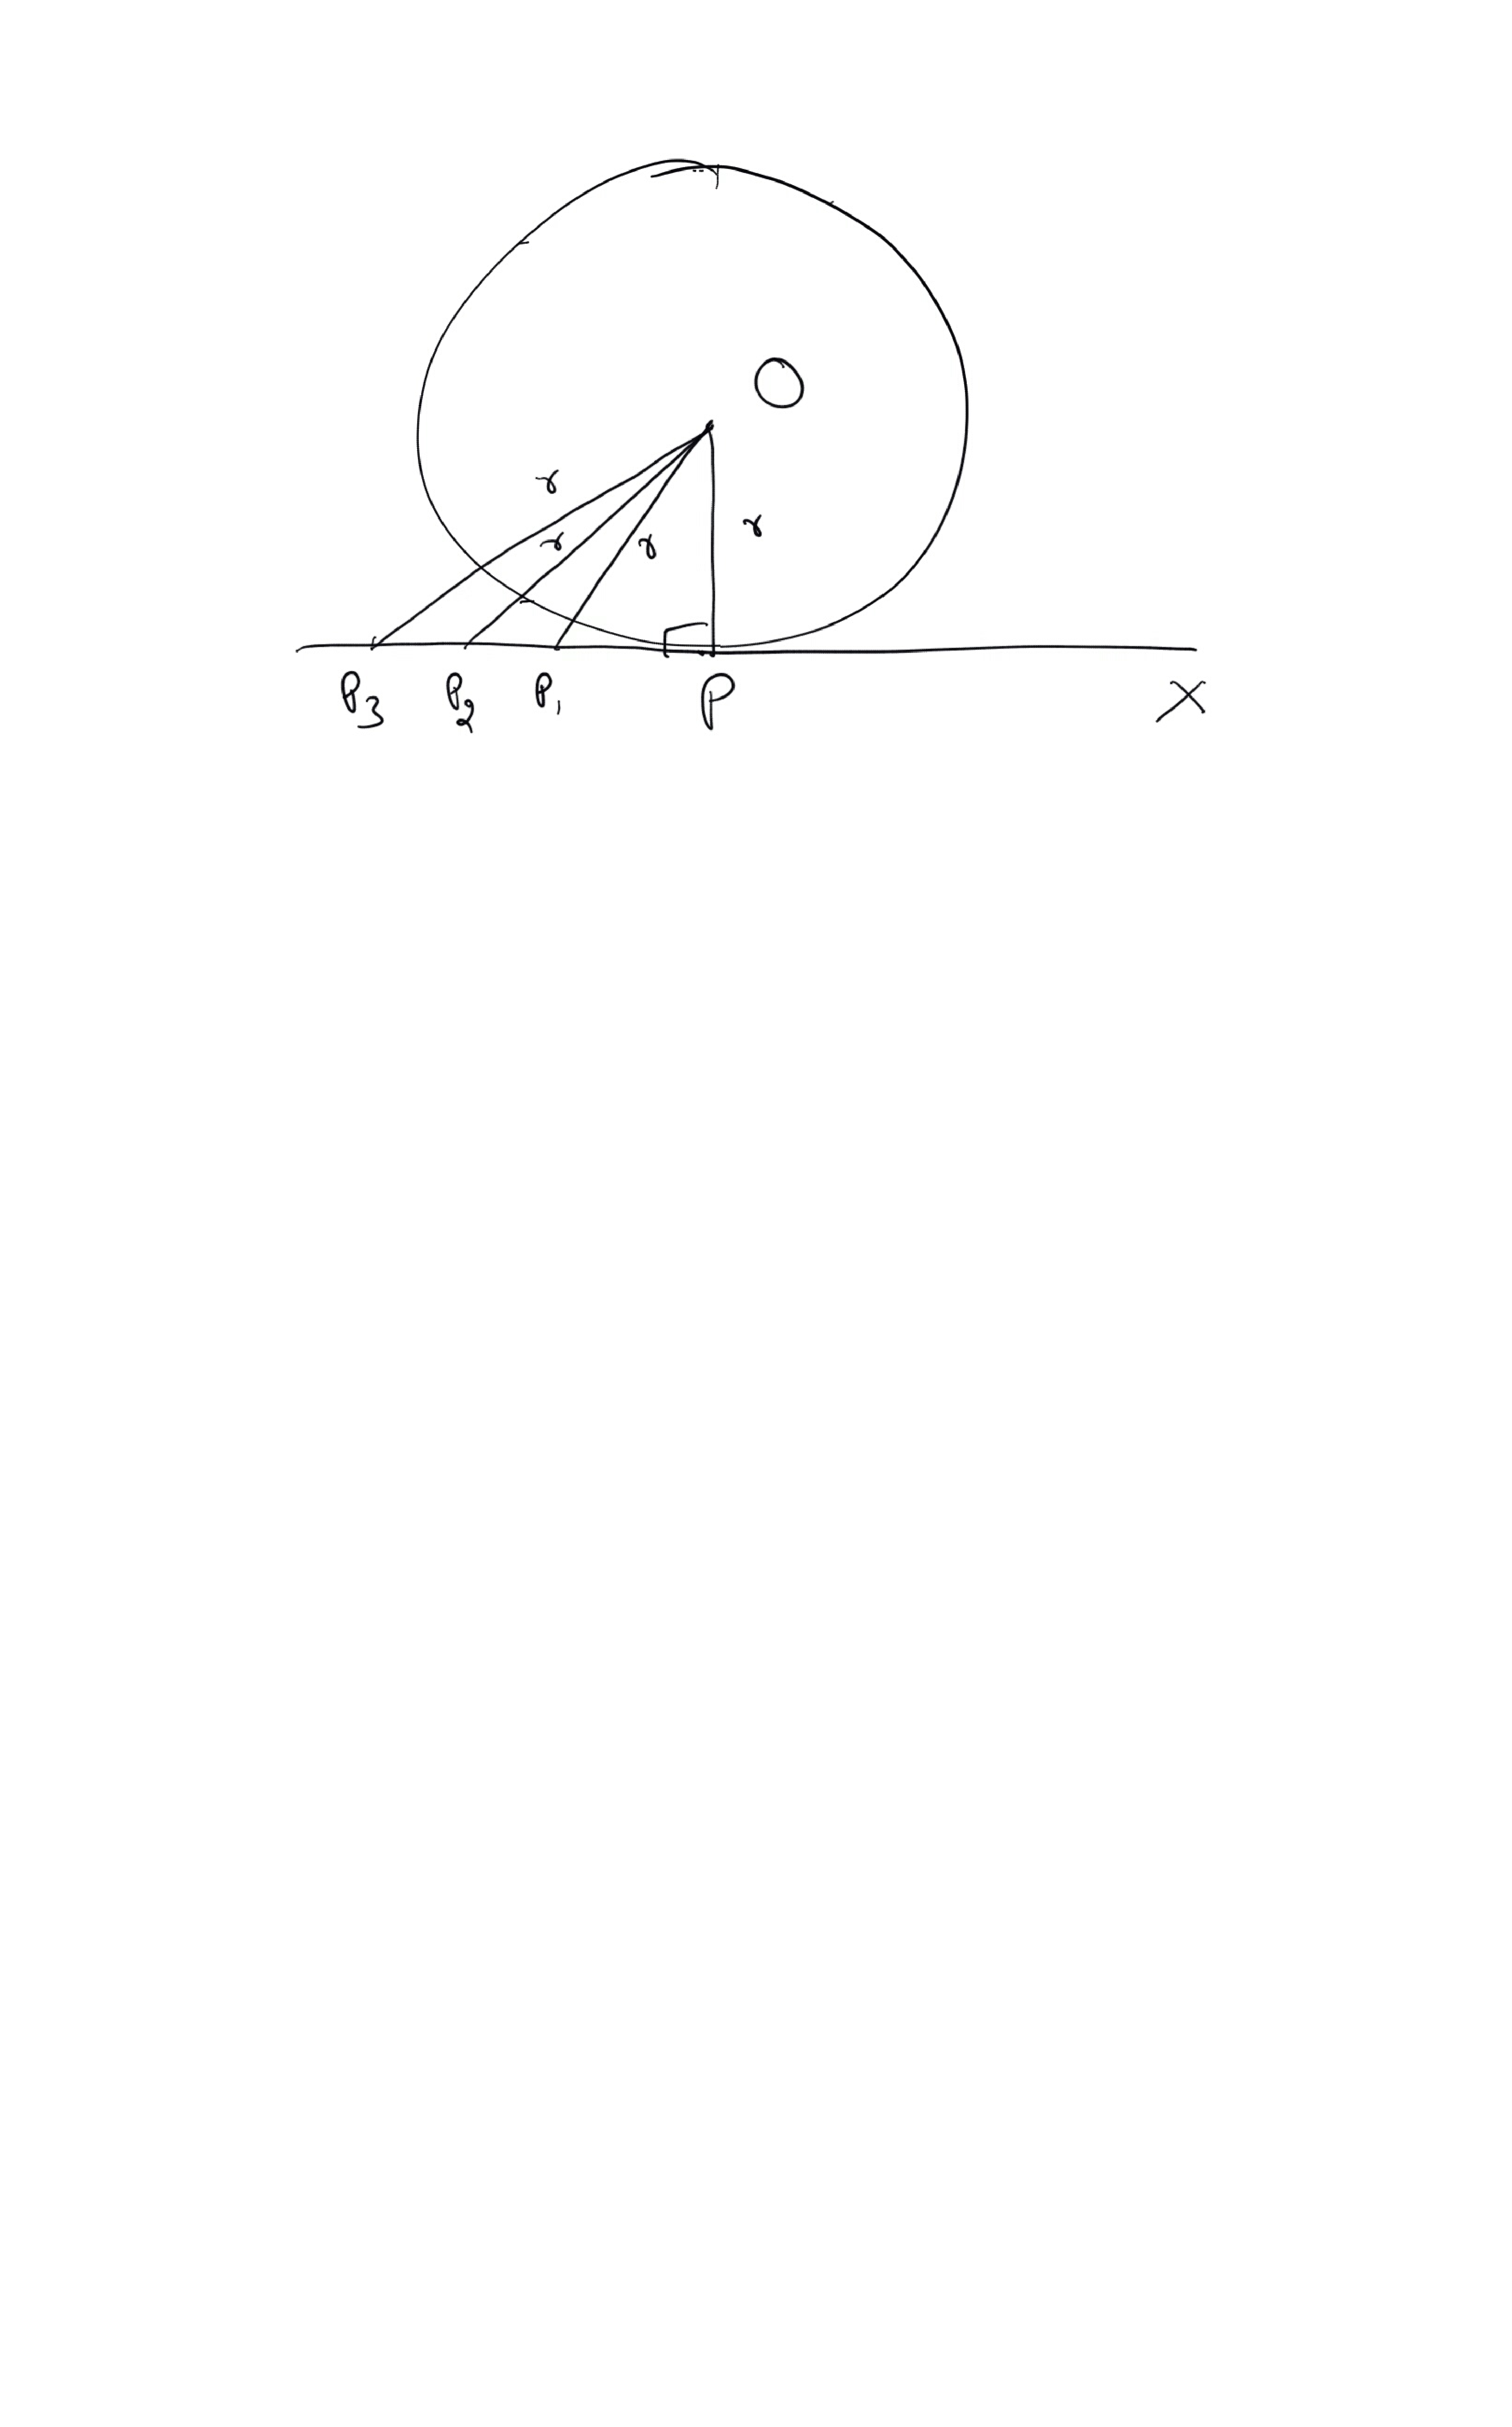
\includegraphics[width=\columnwidth]{./figs/ch4_tangent_def}
		\vspace*{-10cm}
	\end{center}
	\caption{Tangent to a Circle.}
	\label{ch4_tangent_def}	
\end{figure}
%
\begin{figure}[!h]
	\begin{center}
		
		
\includegraphics[width=\columnwidth]{./figs/ch4_short_dist}
		\vspace*{-10cm}
	\end{center}
	\caption{Shortest distance from $O$ to line $PX$}
	\label{ch4_short_dist}	
\end{figure}

%
\begin{equation}
\begin{split}
OP_1^2 &= OP^2 + PP_1^2 \\
\Rightarrow OP_1 > OP
\end{split}
\end{equation}
%
Thus, $OP$ is the shortest distance between $O$ and line $PX$.
%
\begin{problem}
Show that $\angle OPX = 90 ^{\degree}$
\end{problem}
\proof In Fig. \ref{ch4_tangent_def}, we can see that $OP$ is is the radius of the circle and the length of all line segments from $O$ to the line $PX > r$.  Using the result of the previous 
problem, it is obvious that $OP \perp PX$. 
%
	%
\begin{problem}
In Fig. \ref{ch4_tangent_prod} show that 
%
\begin{equation}
\angle PCA = \angle PBC
\end{equation}
%
$O$ is the centre of the circle and $PC$ is the tangent.
\end{problem}
	\begin{figure}[!h]
		\begin{center}
			
			
\includegraphics[width=\columnwidth]{./figs/ch4_tangent_prod}
			\vspace*{-10cm}
		\end{center}
		\caption{$PA.PB = PC^2$.}
		\label{ch4_tangent_prod}	
	\end{figure}
	%

%
\proof For convenience, greek letters are used for representing certain angles. Since $\Delta OAC$ is isosceles,
%
\begin{align}
2 \alpha + 2 \brak{\beta - \phi} &= 180^{\degree} \\
\Rightarrow  \alpha +  \brak{\beta - \phi} &= 90^{\degree} \\
\Rightarrow  \alpha +  \beta  &= 90^{\degree} + \phi
\end{align}
%
Since $theta$ is an exterior angle for the $\Delta ABC
$,
%
\begin{equation}
\theta = \alpha + \beta
\end{equation}
%
From both the above equations
%
\begin{equation}
\theta = 90^{\degree} + \phi
\end{equation}
%
Since PC is the tangent, 
%
\begin{equation}
\angle PCB = 90^{\degree} + \phi = \theta
\end{equation}
%
Considering the sum of angles in $\Delta PAC$ $\Delta PBC$,
%
\begin{align}
\angle P + \theta + \angle PCA &= 180^{\degree} \\
\angle P + \theta + \alpha &= 180^{\degree}
\end{align}
Hence,
%
\begin{equation}
\angle PCA = \alpha
\end{equation}
%
\begin{problem}
	In Fig. \ref{ch4_tangent_prod}, show that the triangles $PAC$ and $PBC$ are similar.
\end{problem}
\proof From the previous problem, it is obvious that corresponding angles of both triangles are equal.  Hence they are similar.
%
\begin{problem}
	Show that $PA.PB = PC^2$
\end{problem}
\proof Since $\Delta PAC \sim \Delta PBC$, their sides are in the same ratio.  Hence,
%
\begin{align}
\frac{PA}{PC} &= \frac{PC}{PB} \\
\Rightarrow PA.PB &=PC^2
\end{align}
%
%
\begin{problem}
	In Fig. \ref{ch4_chord_tangent_prod}, show that\begin{equation}
	PA.PB = PC.PD
	\end{equation}
\end{problem}
%
\begin{figure}[!h]
	\begin{center}
		
		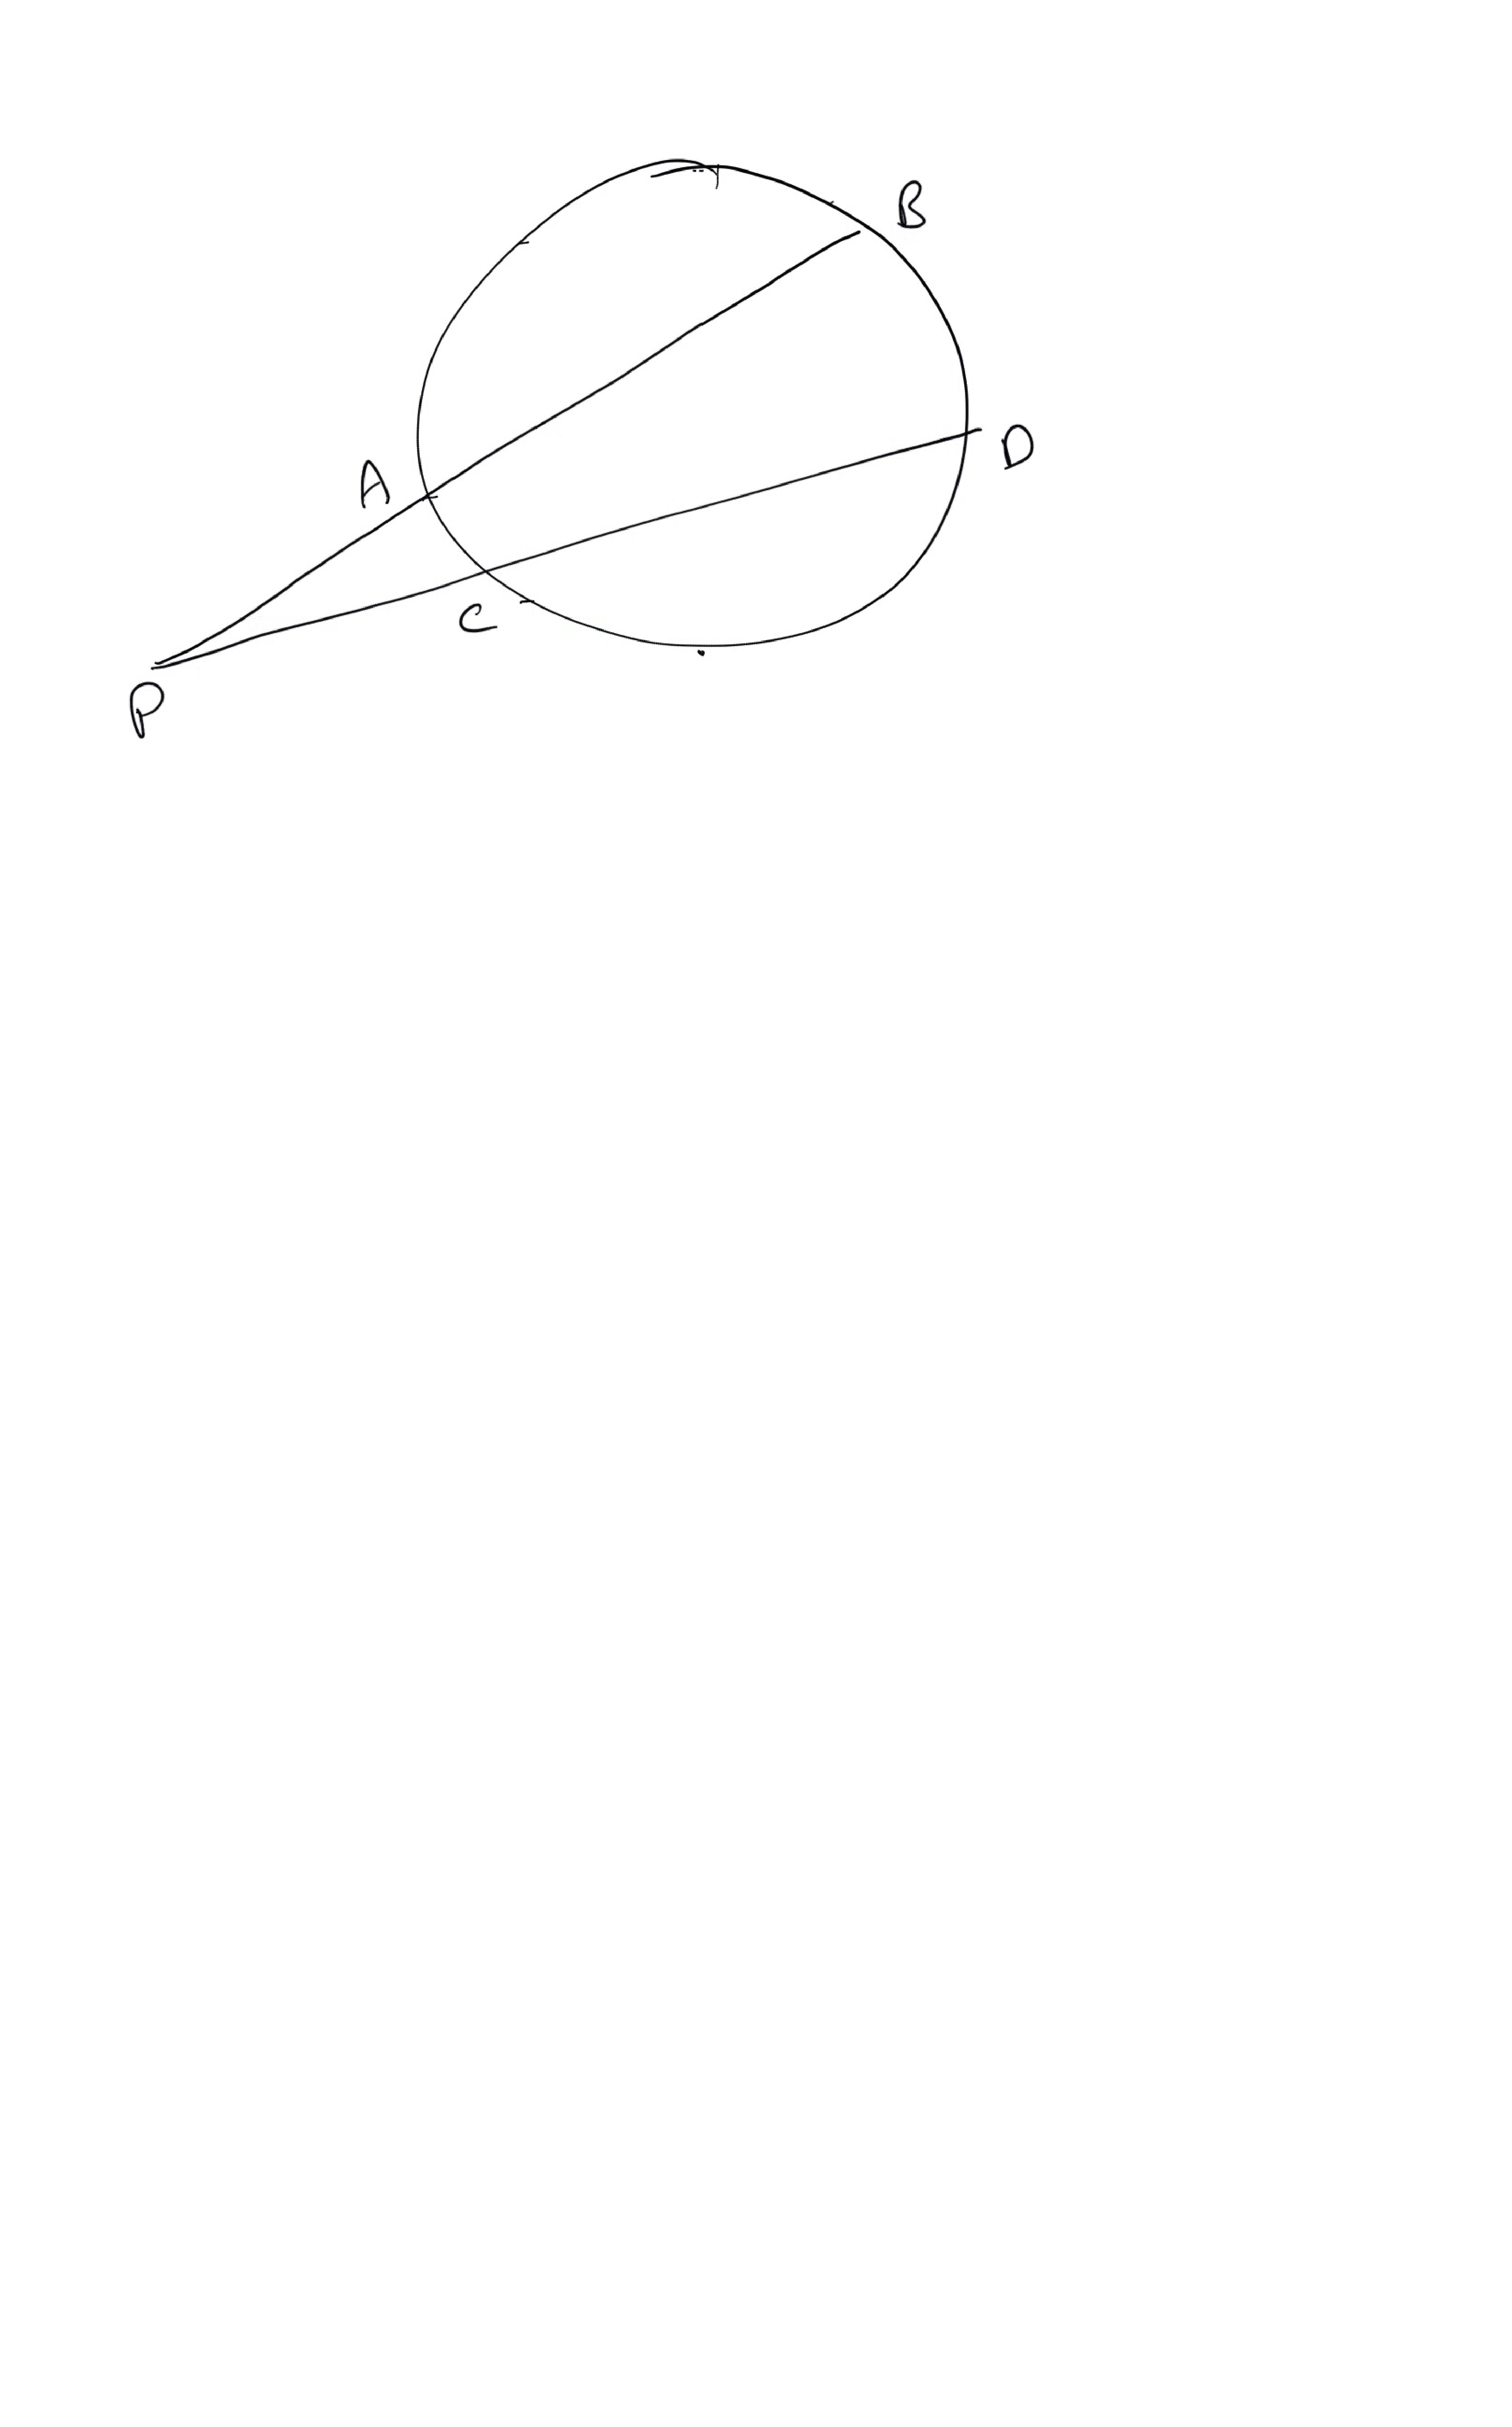
\includegraphics[width=\columnwidth]{./figs/ch4_chord_tangent_prod}
		\vspace*{-10cm}
	\end{center}
	\caption{$PA.PB = PC^2$.}
	\label{ch4_chord_tangent_prod}	
\end{figure}

\proof Draw a tangent and use the previous problem.
 

\end{document}


